% XeLaTeX

\documentclass{article}
\usepackage{ctex}
\usepackage{xypic}
\usepackage{amsfonts,amssymb}
\usepackage{multirow}
\usepackage{geometry}
\usepackage{graphicx}
\usepackage{listings}
\usepackage{lipsum}
\usepackage{courier}
\usepackage{fancyvrb}
\usepackage{etoolbox}


\linespread{1.2}
\geometry{left=3cm,right=2.5cm,top=2.5cm,bottom=2.5cm}

\makeatletter
\patchcmd{\FV@SetupFont}
  {\FV@BaseLineStretch}
  {\fontencoding{T1}\FV@BaseLineStretch}
  {}{}
\makeatother

\lstset{basicstyle=\small\fontencoding{T1}\ttfamily,breaklines=true}
\lstset{numbers=left,frame=shadowbox,tabsize=4}
%\lstset{extendedchars=false}
\begin{document}

\title{实验三 \ 开发独立内核的操作系统 \ 实验报告}
\author {数据科学与计算机学院 \ 计算机科学与技术 2016 级 \\ 王凯祺 \ 16337233}
\maketitle

\section{实验目的}

\begin{itemize}
\item 掌握引导操作系统内核的方法
\item 掌握 C 与汇编交叉调用的方法
\item 掌握汇编程序与 C 程序链接的方法
\end{itemize}

\section{实验要求}

写一个引导程序,能引导操作系统内核。

写一个操作系统内核,可加载多个用户程序。其中,操作系统内核分为汇编模块和 C 模块, C 模块需完成的功能有:

\begin{itemize}
\item 在磁盘上建立一个表,记录用户程序的存储安排
\item 可以在控制台查到用户程序的信息,如程序名、字节数、在磁盘映像中的位置等
\item 设计一种命令,并能在控制台发出命令,执行用户程序等
\end{itemize}

\section{实验步骤}

在本实验中,我使用 NASM 来设计引导程序, TASM + TCC 来设计操作系统内核。

\subsection{设计引导程序}

我使用 NASM 来设计引导程序。引导程序启动后,将操作系统内核加载到 0xA100H ,并跳转到操作系统内核。

在此过程中,我拿老师下发的 showstr.asm 以及 upper.c 作为操作系统内核来启动,却发现启动后无法显示字符,但光标移动了。这时我认为操作系统内核的代码确实执行了,但数据段的数据并没有被成功读取到。

我回忆在 NASM 程序下,可以直接使用 org 0xA100H 来设置所有段的偏移量,所以我尝试在 TASM 下使用 org 0xA100H ,结果链接错误,于是到群里问老师“无法访问内核数据段的数据”该如何解决。我翻了一下班群的消息记录,杂音同学的一句话回答了我的问题:“段值和偏移量错了吧,你读到a100那cs:ip=a00:100”。我意识到数据段 ds 没设置好,就把数据段 ds 设置为 0x0A00H ,数据段就能正常访问了!

以下是引导程序的源代码(NASM 格式):

\begin{lstlisting}[language={[x86masm]Assembler}]
org  7c00h		; BIOS将把引导扇区加载到0:7C00h处,并开始执行
OffSetOfUserPrg1 equ 0a100h
Start:
	mov	ax, cs	       ; 置其他段寄存器值与CS相同
	mov	ds, ax	       ; 数据段
	mov	ax, ds		   ; ES:BP = 串地址
	mov	es, ax		   ; 置ES=DS
	
LoadnEx:
	;读软盘或硬盘上的若干物理扇区到内存的ES:BX处:
	mov bx, OffSetOfUserPrg1  ;偏移地址; 存放数据的内存偏移地址
	mov cx, bx
	mov ah,2                 ; 功能号
	mov al,9                 ;扇区数
	mov dl,0                 ;驱动器号 ; 软盘为0,硬盘和U盘为80H
	mov dh,0                 ;磁头号 ; 起始编号为0
	mov ch,0                 ;柱面号 ; 起始编号为0
	mov cl,2                 ;起始扇区号 ; 起始编号为1
	int 13H ;                调用读磁盘BIOS的13h功能
	; 用户程序a.com已加载到指定内存区域中
	jmp OffSetOfUserPrg1
	
	times 510-($-$$) db 0
	db 0x55,0xaa
\end{lstlisting}

\subsection{设计操作系统内核}

\subsubsection{汇编部分}

汇编部分要完成两方面的任务:

\begin{itemize}
\item 设置数据段
\item 链接到 C 程序入口点
\end{itemize}

我只需把老师提供的 showstr.asm 中 mov ax, cs 替换为 mov ax, 0a00h ,再把 C 函数名替换为我实现的函数名即可。

以下是操作系统内核,汇编部分(TASM 格式):

\begin{lstlisting}[language={[x86masm]Assembler}]
extrn _main:near   ;声明一个c程序函数main
.8086
_TEXT segment byte public 'CODE'
DGROUP group _TEXT,_DATA,_BSS
       assume cs:_TEXT
org 0100h
start:
	mov  ax,  0a00h
	;mov  ax,  cs
	mov  ds,  ax           ; DS = 0a00h
	mov  es,  ax           ; ES = 0a00h
	mov  ax,  0c00h
	mov  ss,  ax           ; SS = 0c00h
	mov  sp, 0ffffh
	call near ptr _main
	jmp $

_TEXT ends
;************DATA segment*************
_DATA segment word public 'DATA'
_DATA ends
;*************BSS segment*************
_BSS	segment word public 'BSS'
_BSS ends
;**************end of file***********
end start
\end{lstlisting}

\subsubsection{C 语言部分}

我找到了一篇《内蒙古科技与经济》2002年第9期其其格写的论文《如何在C语言程序中调用汇编语言》,可以直接在 C 程序中直接嵌入汇编代码。

\paragraph{标准输入输出}

按照 C 语言程序设计规范,输入输出模块我写在 stdio.h 下。

\subparagraph{输出一个字符}

输出一个字符需要考虑:

\begin{itemize}
\item 在当前光标输出字符
\item 输出字符后光标的移动
\item 是否为可见字符
\item 回车需要换行
\item 滚动屏幕
\end{itemize}

这些问题在我的程序都一一解决了。

对于第 1 个问题,我使用 int 10h 中断 0a 功能号,即可在当前光标位置输出字符。

对于第 2 个问题,输出字符后光标的移动。我使用 int 10h 中断 03h 功能号获取当前光标位置。记 $pos = 80x + y$ ,将 pos 加 1 后转换回 $x$ 和 $y$ ,使用 int 10h 中断 02h 功能号设置光标位置。

对于第 3 个问题,在使用 int 10h 的 0a 功能之前加入条件分支判断:如果为可见字符才在当前光标位置输出字符。

对于第 4 个问题,若该字符恰好为回车字符,则下一个光标位置不再是 $pos + 1$ ,而是 $80(x + 1)$ ,即下一行的第 1 个字符。

对于第 5 个问题,若 $pos \geq 2000$ (屏幕大小为 $25 \times 80$ ),则使用 int 10h 的 06h 功能号进行滚屏。

C 语言(内嵌汇编)代码如下:

\begin{lstlisting}[language=C]
void putchar(char c) {
	char x, y;
	int pos;
	
	if (c >= 32) {
		asm mov ah, 0ah
		asm mov al, c
		asm mov bh, 0
		asm mov cx, 1
		asm int 10h
	}
	
	asm mov ah, 03h
	asm mov bx, 0
	asm int 10h
	asm mov x, dh
	asm mov y, dl
	
	if (c == 13)
		pos = (x + 1) * 80;
	else
		pos = x * 80 + y + 1;
	
	if (pos >= 2000) {
		asm mov ah, 06h
		asm mov al, 1
		asm mov bh, 07h
		asm mov dh, 24
		asm mov dl, 79
		asm mov ch, 0
		asm mov cl, 0
		asm int 10h
		pos -= 80;
	}
	x = pos / 80;
	y = pos % 80;
	
	asm mov ah, 02h
	asm mov bh, 0
	asm mov dh, x
	asm mov dl, y
	asm int 10h
}
\end{lstlisting}

\subparagraph{输入一个字符}

从标准输入中输入一个字符,相对于输出一个字符来说简单多了!

我只需要调用 16h 中断 0h 功能号,即可从标准输入中输入该字符。

对于输入后回显字符,只需要在读取完立刻 putchar ,就能实现回显。

C 语言(内嵌汇编)代码如下:

\begin{lstlisting}[language=C]
char getchar() {
	char x;
	asm mov ah, 0
	asm int 16h
	asm mov x, al
	putchar(x);
	return x;
}
\end{lstlisting}

\subparagraph{输入输出字符串}

由于 putchar 、 getchar 函数已经写好,我可以直接调用这些函数来实现输入输出字符串。

C 语言代码如下:

\begin{lstlisting}[language=C]
void gets(char *s) {
	char x = getchar();
	int i = 0;
	for (; x != 13; x = getchar())
		s[i++] = x;
	s[i++] = 0;
}

void puts(const char* s) {
	int i = 0;
	for (; s[i] != '\000'; ++i)
		putchar(s[i]);
	putchar(13);
}
\end{lstlisting}

我有个不明白的地方,gets 和 puts 传进来的指针一定要是 C 语言中全局变量的字符数组的头指针;如果在一个函数中定义一个字符数组,这个指针传进来时指向的不是预期的位置。例如:

\begin{lstlisting}[language=C]
void test() {
	char st[100];
	st[0] = 'a';
	st[1] = 'b';
	st[2] = '\000';
	puts(st);
}
\end{lstlisting}

由于 st 数组是在 test() 函数内,st 的头指针输入到 puts 里就会发生错误,我至今还不知道为什么,一度怀疑我写的是假的 C 。根据我多年的编程经验,我尝试把数组移到函数外。结果令人意外的是,问题就不再出现了:

\begin{lstlisting}[language=C]
char st[100];

void test() {
	st[0] = 'a';
	st[1] = 'b';
	st[2] = '\000';
	puts(st);
}
\end{lstlisting}

\paragraph{字符串函数}

我实现了两个比较常用的字符串函数:strlen, strcmp。

strlen 用于取字符串长度。

strcmp 用于比较两个字符串的大小,若 a < b, 返回 -1 ;若 a = b ,返回 0;若 a > b ,返回 1 。

\begin{lstlisting}[language=C]
int strlen(char *s) {
	int i = 0;
	while (s[i]) ++i;
	return i;
}

int strcmp(char *a, char *b) {
	int la = strlen(a);
	int lb = strlen(b);
	int i = 0;
	for (; i < la || i < lb; ++i)
		if (a[i] > b[i])
			return 1;
		else if (a[i] < b[i])
			return -1;
	return 0;
}
\end{lstlisting}

\paragraph{读取用户程序信息}

我的用户程序信息存储在 11 号扇区, 0x1400 位置,格式是一个字符串表示程序名,然后是一个数字表示扇区号。如有多个程序,则将上述格式重复若干次。

读取用户程序信息时,我使用 int 13h 的 02h 功能号来读取 11 号扇区的数据,得到某程序的扇区号后,再次使用 int 13h 的 02h 功能号读取该扇区数据,计算出这个程序占用的字节数。

以下是 C 语言(内嵌汇编)代码:

\begin{lstlisting}[language=C]
int get_file_size(int id) {
	char tmp;
	int i = 0, j = 0, addr;
	asm mov bx, 8400h
	asm mov ah, 2
	asm mov al, 1
	asm mov dl, 0
	asm mov dh, 0
	asm mov ch, 0
	asm mov cl, id
	asm int 13h
	asm mov ax, 8400h
	asm mov addr, ax
	for (i = 0; i < 512; ++i) {
		asm mov bx, addr
		asm mov al, [bx]
		asm mov tmp, al
		asm inc bx
		asm mov addr, bx
		if (tmp != 0)
			j = i + 1;
	}
	return j;
}

void ls() {
	char tmp;
	int size, i, j, k, addr;
	asm mov bx, 8000h
	asm mov ah, 2
	asm mov al, 1
	asm mov dl, 0
	asm mov dh, 0
	asm mov ch, 0
	asm mov cl, 11
	asm int 13h
	
	asm mov ax, 8000h
	asm mov addr, ax
	puts("===============================");
	puts_format("Filename", 15);
	putchar('|');
	puts_format("Sector", 10);
	putchar('|');
	puts("Size");
	puts("-------------------------------");
	for (i = 0; ; ++i) {
		j = 0;
		asm mov bx, addr
		asm mov al, [bx]
		asm mov tmp, al
		asm inc bx
		asm mov addr, bx
		while (tmp) {
			st[j] = tmp;
			asm mov bx, addr
			asm mov al, [bx]
			asm mov tmp, al
			asm inc bx
			asm mov addr, bx
			++j;
		}
		st[j] = '\000';
		if (j == 0) break;
		asm mov bx, addr
		asm mov al, [bx]
		asm mov tmp, al
		asm inc bx
		asm mov addr, bx
		puts_format(st, 15);
		putchar('|');
		printint_format(tmp, 10);
		putchar('|');
		size = get_file_size(tmp);
		printint(size);
	}
	puts("===============================");
}
\end{lstlisting}

\paragraph{执行用户程序}

将用户程序从磁盘加载到内存的 9100h 位置,先保存 es 、 ds ,再 call 9100h 。程序返回后,还原 es 、 ds 。

我尝试过 call es:9100h 、 call es:9000h ,都没办法执行用户程序。我必须把 9100h 写入 ax 中,然后 call es:ax 来调用它。我并不知道为什么会这样……

\begin{lstlisting}[language=C]
void execute(int id) {
	puts_format("find at sector ", 0);
	printint(id);
	asm push es
	asm mov ax, 0h
	asm mov es, ax
	asm mov bx, 9100h
	asm mov ax, id
	asm mov cl, al
	asm mov ah, 2
	asm mov al, 1
	asm mov dl, 0
	asm mov dh, 0
	asm mov ch, 0
	asm int 13h
	asm pop es
	
	asm push es
	asm push ds
	asm mov ax, 0h
	asm mov es, ax
	asm mov ax, 9100h
	asm call es:ax
	asm pop ds
	asm pop es
}
\end{lstlisting}

\paragraph{主函数 main}

主函数主要是判断用户的输入,并指挥操作系统作出相应的行为。

比如输入 help ,显示帮助提示;输入 exit ,退出操作系统;输入 ls ,显示程序列表;输入程序名,执行程序等等。

\begin{lstlisting}[language=C]
main(){
	welcome();
	while (1) {
		puts_no_new_line("$ ");
		gets(cmd);
		if (strcmp(cmd, "") == 0) {
		} else
		if (prefix_match(cmd, "help")) {
			help();
		} else
		if (prefix_match(cmd, "exit")) {
			return;
		} else
		if (prefix_match(cmd, "ls")) {
			ls();
		} else
		if (find_exe()) {
			
		} else {
			puts("command not found");
		}
	}
}
\end{lstlisting}

\subsection{编译与链接}

编译引导程序:

\begin{lstlisting}[language=bash]
nasm -f bin myos.asm -o myos.com
\end{lstlisting}

编译和链接操作系统内核:

\begin{lstlisting}[language=bash]
tasm loader.asm loader.obj
tcc -mt -c -omain.obj main.c
tlink /3 /t loader.obj main.obj,loader.com,,
\end{lstlisting}

\subsection{写入磁盘文件}

将 myos.com 写入 1 号扇区(0x0000 位置);

将 loader.com 写入 2 号扇区(0x0200 位置);

将用户程序信息写入 11 号扇区(0x1400 位置);

将用户程序写入 12 号及以后扇区的位置。

\newpage 

\section{实验结果}


\begin{figure}[!hbp]
	\centering
	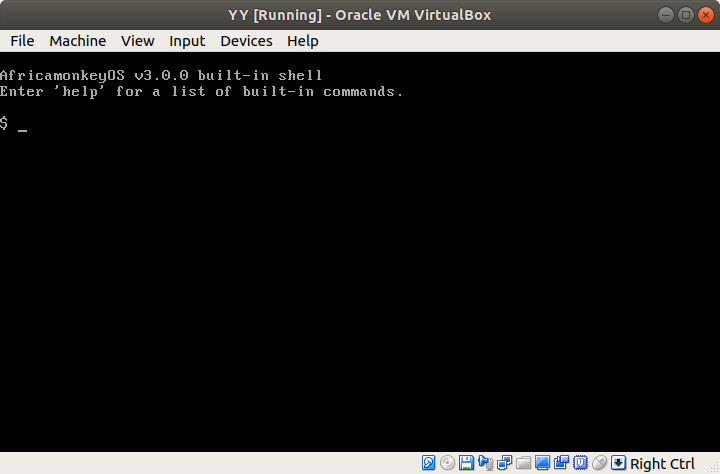
\includegraphics[scale=0.55]{pics/1.png}
\end{figure}

上图显示,我的引导程序能正确地将操作系统内核加载到指定位置,并启动操作系统内核。上图的信息是由操作系统内核输出的。

\begin{figure}[!hbp]
	\centering
	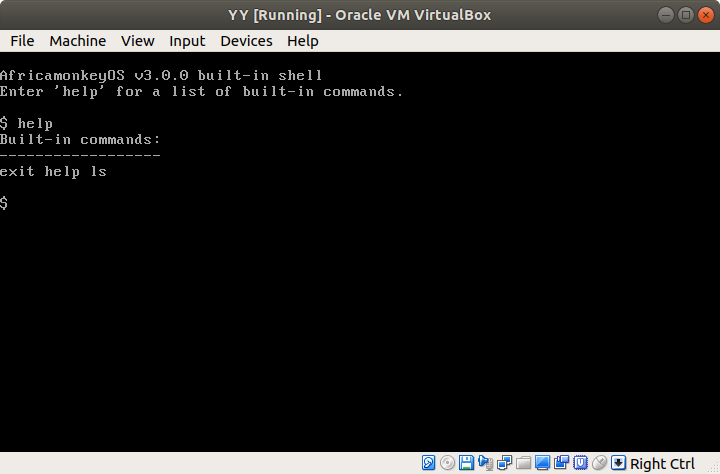
\includegraphics[scale=0.55]{pics/2.png}
\end{figure}

上图展示的是 help 功能。输入 help 将会列出操作系统支持的所有指令。

\newpage

\begin{figure}[!hbp]
	\centering
	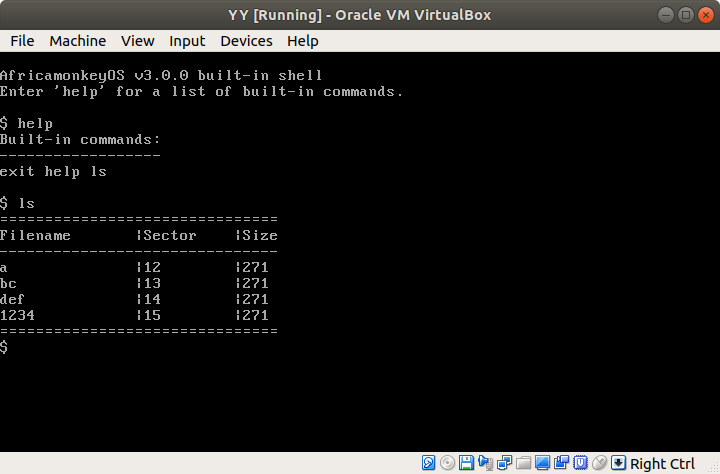
\includegraphics[scale=0.55]{pics/3.png}
\end{figure}

上图展示的是显示用户程序信息的功能。输入 ls 会显示磁盘里用户程序的文件名、扇区号和程序大小。

\begin{figure}[!hbp]
	\centering
	
\includegraphics[scale=0.55]{pics/4.png}
\end{figure}

上图展示的是执行用户程序功能。输入用户程序的文件名,将会执行用户程序。

\newpage

\begin{figure}[!hbp]
	\centering
	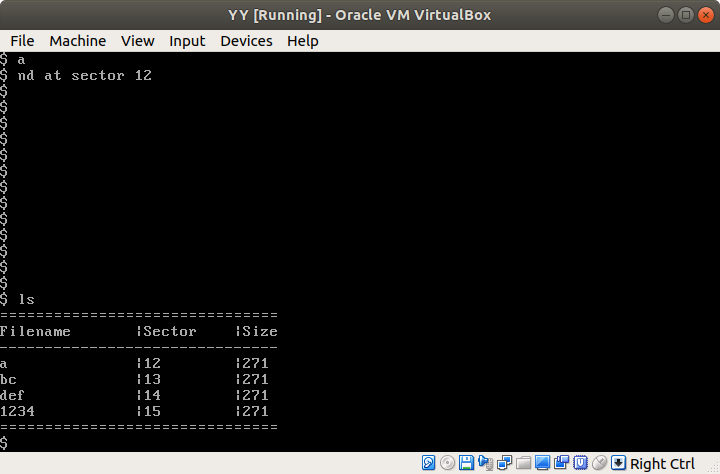
\includegraphics[scale=0.55]{pics/5.png}
\end{figure}

上图展示的是执行用户程序后回到操作系统的功能。用户程序执行 ret 指令,将由操作系统接管控制权,可继续执行其他指令。

\begin{figure}[!hbp]
	\centering
	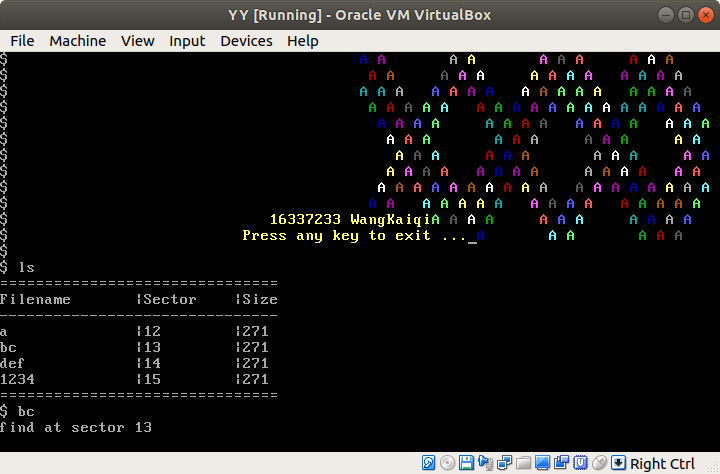
\includegraphics[scale=0.55]{pics/6.png}
\end{figure}

上图展示的是执行用户程序功能。输入用户程序的文件名,将会执行用户程序。

\newpage



\section{实验总结}

这次实验耗费了我不少时间,但最终能圆满完成,我觉得很值得。

在这次实验中,我终于理解了汇编语言的 4 个段(CS, DS, ES, SS)分别起何作用。CS 段是程序执行的段空间。 设计者将 $CS:IP$ 定义为 $CS * 16 + IP$ ,意在使 16 位程序能使用 20 位(1 MB)的空间。DS 段是数据存储的段空间,使用 jmp 或 call 指令执行其他程序,需要自行修改 ds 寄存器,使得段地址加上偏移地址恰好等于程序加载的地址,这样就能访问数据段了。而 ES 段在中断程序会用到,比如读写磁盘加载到内存的位置用 ES:BX 表示。

这个实验有很多个瓶颈问题,我列举一下:

\begin{itemize}
\item 加载 TASM 编写的操作系统内核
\item 读取软盘文件特定的一个字节
\item 用 TASM 加载用户程序
\end{itemize}

对于第一个,加载 TASM 编写的操作系统内核,难点在于正确设置数据段。只要弄清楚了程序的工作原理,这个问题就解决了。这个问题困扰了我很久,我在 Google 查了很多相关的资料,都没有对于该问题的解释。也许是因为我对问题的分析不够透彻,搜索的关键字没有到点子上。这个问题群里很多同学都遇到过,非常感谢杂音同学明确地指出问题,并提供解决方案。

对于第二个,读取软盘文件中特定的一个字节。首先把软盘的整个扇区加载到内存中,这个大家都会。但如何读取到内存中的那一个字节呢?有时我会怀疑 DS 、 ES 是否设置错误,反反复复改了很多次。经过多次测试,我终于知道应该先将立即数存到 ax 中,然后 [ax] 的值就是要读取的那个字节。

对于第三个,我同样也是反反复复尝试了很多次。设程序加载到 9100h 位置,我尝试过跳转到立即数 jmp 9100h 、跳转到立即数 jmp 9000h ;试过先把 9100h 写入 ax ,再 jmp ax ;试过把 900h 写入 es ,再 jmp es:100h ;试过把 0h 写入 es ,再 jmp es:9100h ;最后尝试将 0h 写入 es ,将 9100h 写入 ax ,再 jmp es:ax ,成功。只有坚持不断尝试,才有可能成功。

\end{document}
















